% TikZ plot for 2025_vggnet16_2022
% Generated automatically with embedded data
% Requires: \usepackage{pgfplots} \pgfplotsset{compat=1.18}

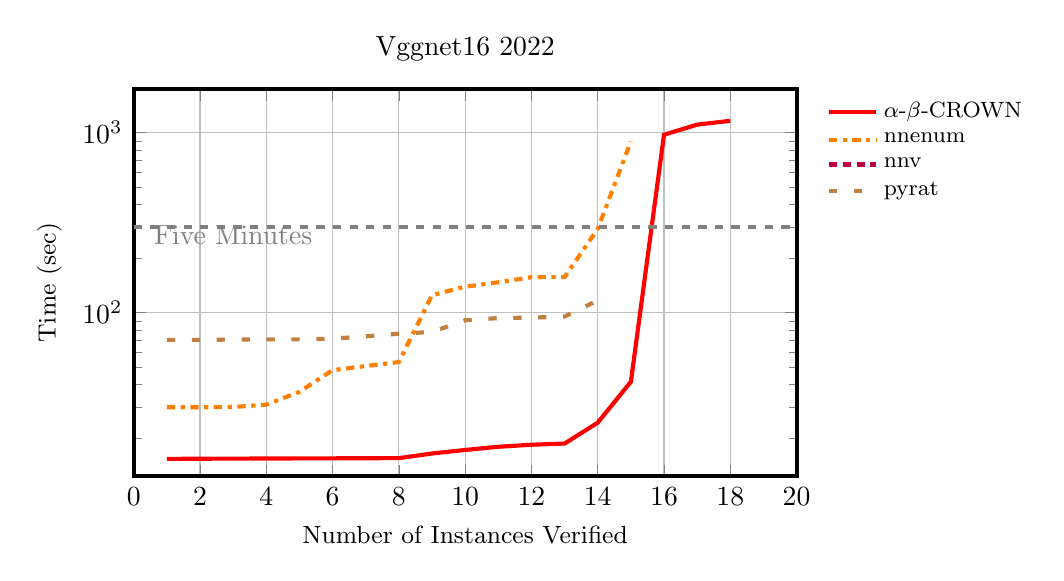
\begin{tikzpicture}
\begin{semilogyaxis}[
    xlabel={Number of Instances Verified},
    ylabel={Time (sec)},
    legend pos=outer north east,
    grid=major,
    width=10cm,
    height=6.5cm,
    ymin=12.324,
    ymax=1747.5,
    xmin=0,
    xmax=20,
    line width=1.5pt,
    legend style={font=\footnotesize, cells={anchor=west}, draw=none},
    xlabel style={font=\small},
    ylabel style={font=\small},
    title={Vggnet16 2022},
    title style={font=\normalsize}
]

\addplot[color=red, mark=none, solid] coordinates {
    (1,15.405565)
    (2,15.448401)
    (3,15.464191)
    (4,15.484712)
    (5,15.508128)
    (6,15.519229)
    (7,15.551150)
    (8,15.555607)
    (9,16.514415)
    (10,17.278112)
    (11,17.994776)
    (12,18.469749)
    (13,18.750970)
    (14,24.496119)
    (15,41.314874)
    (16,974.346412)
    (17,1109.058780)
    (18,1164.998963)
};
\addlegendentry{$\alpha$-$\beta$-CROWN}

\addplot[color=orange, mark=none, dashdotted] coordinates {
    (1,29.817439)
    (2,29.849050)
    (3,29.931066)
    (4,30.839708)
    (5,36.338682)
    (6,47.922080)
    (7,50.566527)
    (8,53.176262)
    (9,125.165391)
    (10,139.562398)
    (11,147.515491)
    (12,157.589109)
    (13,157.616845)
    (14,292.252125)
    (15,893.779531)
};
\addlegendentry{nnenum}

\addplot[color=purple, mark=none, densely dashed] coordinates {
    (1,62.056275)
};
\addlegendentry{nnv}

\addplot[color=brown, mark=none, loosely dashed] coordinates {
    (1,70.647094)
    (2,70.665150)
    (3,70.907137)
    (4,71.068144)
    (5,71.120668)
    (6,71.734862)
    (7,73.926419)
    (8,76.429094)
    (9,78.188179)
    (10,90.755872)
    (11,93.352773)
    (12,93.898409)
    (13,95.218734)
    (14,117.052884)
};
\addlegendentry{pyrat}

% Timeout line
\addplot[color=gray, dashed, mark=none, domain=0:20] {300};

% Add timeout label as text below the line
\node[color=gray] at (axis cs:3,270.0) {Five Minutes};

\end{semilogyaxis}
\end{tikzpicture}
